
\documentclass [11pt]{report}

\usepackage{fancyhdr}
\usepackage [french]{babel}

\usepackage[utf8]{inputenc}
\usepackage[T1]{fontenc}
\usepackage{textcomp}
\usepackage{graphicx}
\usepackage[a4paper]{geometry}
\usepackage{titlepic}
\usepackage{boxedminipage}
\usepackage{listings}
\usepackage{minitoc}
\usepackage{footmisc}
\usepackage{color}
\usepackage{graphicx}
\usepackage{fancyvrb}

\usepackage{eso-pic}

\makeatletter
\newlength\@tempdim@x
\newlength\@tempdim@y
% structure des commandes :
%   #1 = deplacement selon x
%   #2 = deplacement selon y
%   #3 = texte à mettre
\newcommand\AtUpperLeftCorner[3]{%
\begingroup
\@tempdim@x=0cm
\@tempdim@y=\paperheight
\advance\@tempdim@x#1
\advance\@tempdim@y-#2
\put(\LenToUnit{\@tempdim@x},\LenToUnit{\@tempdim@y}){#3}%
\endgroup
}
\newcommand\AtUpperRightCorner[3]{%
\begingroup
\@tempdim@x=\paperwidth
\@tempdim@y=\paperheight
\advance\@tempdim@x-#1
\advance\@tempdim@y-#2
\put(\LenToUnit{\@tempdim@x},\LenToUnit{\@tempdim@y}){#3}%
\endgroup
}
\newcommand\AtLowerLeftCorner[3]{%
\begingroup
\@tempdim@x=0cm
\@tempdim@y=0cm
\advance\@tempdim@x#1
\advance\@tempdim@y#2
\put(\LenToUnit{\@tempdim@x},\LenToUnit{\@tempdim@y}){#3}%
\endgroup
}
\newcommand\AtLowerRightCorner[3]{%
\begingroup
\@tempdim@x=\paperwidth
\@tempdim@y=0cm
\advance\@tempdim@x-#1
\advance\@tempdim@y#2
\put(\LenToUnit{\@tempdim@x},\LenToUnit{\@tempdim@y}){#3}%
\endgroup
}
% ajout de texte ou d'images en haut à gauche, en haut à droite, etc.
\AddToShipoutPicture{%
\AtLowerRightCorner{3cm}{1cm}{
\includegraphics[scale=0.20]{images/LogoGroupe.png}}% image en bas à droite
}
\makeatother

\pagestyle{fancy}





\title{
	
\includegraphics[scale=0.43]{images/Logojeu.png}
	 \\\vspace{20mm}
	\textbf{\Huge \itshape Rapport de premi\`ere soutenance  }
	}




\author{ \\\vspace{2mm}
	Thibault Gdalia\\\vspace{2mm}
	Florent Youinou\\\vspace{2mm}
	Mathilde Laplaze\\\vspace{2mm}
	Vincent Baille \\\vspace{30mm}
	}


\date{17 janvier 2014}


\usepackage{listings,mdframed,xcolor}
\definecolor{codeBackground}{rgb}{0.95, 0.95, 0.95} %Couleur du rectangle%


\lstnewenvironment{mylisting}{
  \lstset{
  }
  \mdframed[backgroundcolor=codeBackground,shadow=false,shadowsize=2pt,shadowcolor=black!30]
}
{
  \endmdframed\ignorespaces
}


\begin{document}
\thispagestyle{fancy}
\renewcommand{\baselinestretch}{0.001}
\maketitle
\tableofcontents

\newpage



\chapter*{Introduction}
\addcontentsline{toc}{chapter}{Introduction}

\indent Nous sommes la Team Girafe. Un groupe de 4 étudiants composé de Mathilde "Mattou" Laplaze, Vincent "Vincae" Baille, Florent "T4ze" Youinou, Thibault "Skeat" Gdalia. \\\\
\indent Nous produisons actuellement un runner 2D, où le joueur parcourt nos maps à l'aide d'un Houla-Houla. Cet animal est un oiseau très gourmand, qui à chaque effort, consomme de l'énergie, sous forme de sucre. Mais étant donné que cette énergie lui est nécessaire pour voler, des bonbons sont parsemés tout au long de son parcours et son taux de sucre augmente avec le temps.\\
\indent Le jeu est composé de différents modes. Le mode solo où vous devez parcourir les différentes maps attention que votre oiseau reste à l'écran car si il disparait par la gauche : c'est perdu. Le mode multijoueur où la map est infinie et le but est donc d'aller le plus loin possible, le score étant comptabilisé selon le nombre de mètres parcourus, une fois que vous êtes mort (ça arrive à tous un jour malheureusement). Ce score est ensuite envoyé à la base de données de notre site web afin de pouvoir consulter le classement des joueurs.\\

Lors de la création de notre groupe de projet, nous ne savions pas vraiment à quoi nous attendre. Y aurait-il une bonne cohésion de groupe, une bonne entente générale ? C'est lors du commencement du projet que tout cela s'est concrétisé, la motivation s'est avérée être notre point fort. Malgré les différents niveaux d'informatique de chacun, l'entraide nous a permis de mener cette première partie de projet dans de très bonnes conditions. Nous avons ainsi pu accéder à nos attentes sans problèmes de timing.

Nous somme donc en mesure de vous dévoiler une premier version de CandyBird qui est dès à présent jouable et (d'après nous) pas désagréable à regarder. Bien entendu de nombreuses améliorations arriveront par la suite mais grâce à cette version, vous pouvez patienter sans vous ennuyer jusqu'à la version final.\\


Voici donc la présentation et le détail de cette première version accompagnée de nos provisions/ambitions pour la suite.




\chapter{Avancement du Projet}
	\section{Différents modes}
	Dans Candy bird il existe deux modes de jeu, un story mode et infini mode. L'un permet de suivre une succession de maps que nous avons cr\'e\'ee tant dis que l'infini mode vous permet de voir qui est le plus fort entre vous et vos amis.
	
	\vspace{10mm}
	
		\subsection{Mode Histoire}	
		Nous avons créé différente maps qui se jouent les unes après les autres, elles sont de plus en plus dures vous  offrant de plus en plus de challenges au fur et \'a mesure que vous avancez dans le jeu. Ce mode de jeu vous permet de jouer lorsque vous n'avez pas de connexion internet ou si vous n'avez pas encore cr\'ee votre compte sur notre site web. C'est le vrai mode solo de notre jeu car les autres formes de CandyBird sont plus ou moins des modes multijoueurs. Le principe est simple, lorsque vous commencez une partie, vous surmontez les différents obstacles se trouvant sur votre chemin, en pensant \`a régulièrement manger des bonbons pour avoir suffisamment d'énergie pour continuer de voler. A la fin vous verrez une ligne d'arriv\'ee, mais rien \`a voir avec les damiers que l'on voit d'habitude, Nous avons mis une ligne de petits bonbons allant du haut en bas de l'écran.\\
		\\
		\indent
		Il n'y aura pas de grande révolution d'ici la prochaine soutenance, mis \`a part que toutes les maps ne seront pas accessibles d\`es le début du jeu. C'est a dire que si vous voulez accéder \`a la map 43 il faudra finir la map 42, cela parait logique. mis \`a part ca nous ne voyons pas la nécessite de faire de plus grand changement car ce mode de jeu est déjà bien complet et les autres mode de jeu vous permettront de vous amuser de façon plus approfondie dans CandyBird.
		
		\vspace{10mm}
		
	
		\subsection{Mode Infini}
		Ce qui caractérise le mode infini c'est qu'il n'as pas de fin (d'ou son nom). Les maps suivent le même modèle que dans l'autre mode sauf qu'au lieu de charger le contenu d'un fichier, la gestion des blocs se fait de façon aléatoire. Pour ne pas se retrouver avec un parcours infranchissable, la création suit un pourcentage fixé :\\
		
		\indent \indent - 13\% d'obstacles, avec différentes possibilitées de passage.\\
		\indent \indent - 3\% de bonbons, car il ne faut pas que le joueur puisse tout le temps avoir de \indent \indent l'énergie.\\
		\indent \indent - le reste du pourcentage deviens un bloc vide/invisible dans lequel l'oiseau pourra\\
		\indent \indent passer\\
		
			
		Pour ce mode, il ne fallait pas un tableau de largeur infinie (ce n'est d'ailleurs pas possible), nous avons donc créé un tableau de blocs, un peu plus grand que la largeur de la fenêtre puisque nous n'avons pas besoin de plus. Le procédé est simple, à chaque fois qu'une colonne franchis l'écran par la gauche, cela signifie que le bloc à disparut. On modifie donc sa position pour le faire réapparaitre par la droite lors du scrolling. Bien évidemment on change aussi la valeur du bloc en suivant nos pourcentages sinon notre map ne serait composée que d'une même partie qui se répète.


	\vspace{15mm}


	\section{Moteur Physique}
		Dans un runner 2D, le moteur physique est en quelque sorte la base. L'oiseau doit être attiré par le sol, et doit être bloqué par les obstacles. Il était donc naturel que nous en fassions notre plus grand centre d'attention durant cette première partie de projet. Nous avons fait en sorte qu'il soit efficace et que l'on puisse le moduler aisément afin de pouvoir s'amuser à changer les propriétés physiques d'une map à l'autre. Par exemple, la gravité est appliquée au personnage selon un coefficient variable qui peut être modifié en fonction du niveau de difficulté. Le vol  de l'oiseau peut donc être contrôlé, tout comme ses battements d'ailes qui le font avancer en même temps qu'il s'élève dans les airs. \\\\
		
		\indent Étant donné que la carte de jeux a les mêmes dimensions que la fenêtre, la gestion du dépassement de map a été très simple à réaliser. Un simple test sur la position du personnage par rapport à la fenêtre nous permet donc de l'empêcher de voler plus haut que le bord supérieur, ou de tomber plus bas que le bord inférieur. \\


	\newpage
		\noindent Exemple :
		
		\begin{mylisting}
		
if(SpritePosition.Y <= ScreenHeight)
{
	   On peut bouger verticalement l'oiseau
}
else
{
	   On laisse l'oiseau a sa position
}
		\end{mylisting}
	\vspace{10mm}
		
				
		\indent Du côté de la gestion des obstacles, nous les avons faits sous forme de rectangles qui contiennent les images des blocs. Nous avions dans un premier temps implémenté une collision basique, rectangulaires, qui fonctionnait avec ces rectangles. Cette collision fonctionnait assez bien mais notre oiseau est rond, et les images des obstacles ne sont pas forcément rectangulaire non plus, ce n'était donc pas la solution la plus optimale... \\
		\indent Pour remédier à ce problème, l'idée nous est donc venue de passer par une collision par pixel, bien plus adaptée à l'utilisation que l'on en fait dans notre jeu. Le problème de cette collision, c'est qu'elle est très gourmande puisque même en étant optimisée au maximum, elle parcourt beaucoup de pixel. Il a donc fallu assembler les deux tests, collision rectangulaire puis par pixel afin de ne pas tester une collision par pixel avec le rectangle d'un bloc si il ne touche pas le rectangle du personnage. car si il n'y a pas d'obstacle nous n'avons donc pas besoin de regarder si il y a une collision à gérer, de plus nous n'avons pas besoin de gérer la collision de façon optimale pour les bonbons, donc pas besoin de perdre du temps machine pour quelque chose qui ne nous sert pas, soyons logique. Pour résumer nous avons fait un mix des deux grandes sortes de collisions (on est des oufs, ou pas...)
		
		\newpage
	
	\section{Son}
		Nous savons que tout bon jeu est accompagné d'une vraie bibliothèque de sons, c'est pourquoi Mattou s'est vraiment concentrée sur cet aspect du projet, il a fallu tout d'abord qu'elle recherche les musiques et les effets sonores adéquats pour que l'ambiance lorsque vous êtes dans le jeu soit optimale. Puis nous voulions que ce soit très structuré dans le projet pour ne pas avoir des sons en vrac dans nos Contents, notre solution: utiliser Xact. \\
		
	\indent Nous nous sommes très vite mis d'accord sur ce que nous recherchions comme ambiance, et Mattou s'est chargée à-partir de là  de trouver les pistes. Elle s'est donc inspirée d'autres Runner 2D pour les pistes jouées pendant la partie. Il n'y a pour l'instant que peu de maps, donc une piste par maps pour chaque maps du jeu. D'autres viendront par la suite, accompagnées de nouvelles pistes respectives. Les autres états de jeu ont également leur propre musique. \\
	
	
	\indent Une fois les sons trouvés et approuvés, il a fallu les implémenter. Ce ne fut pas une partie de plaisir car Mattou ne connaissait pas Xact et ses méthodes. De plus, une fois le son implémenté, nous nous sommes rendus compte que les pistes étaient trop importantes et mettaient du temps à se lancer dans le jeu. Le rendu n'étant pas satisfaisant, il a fallu compresser chaque piste dans l'API Xact. Et voilà, nous avons du son dans le jeu ! Peut être que certains morceaux seront remplacés ou modifiés afin qu'ils s'accordent mieux entre eux, mais nous nous occuperons de cette partie lorsque le projet aura évolué et que nous aurons plus de maps. Des sons vont  également arriver plus tard, pour le déroulement de la partie (par exemple lorsque l'oiseau attrape un bonbon, ou que la barre de vie est presque vide...).

		\vspace{8mm}
		
		\begin{minipage}[c]{.45\linewidth}
		\begin{center}h
		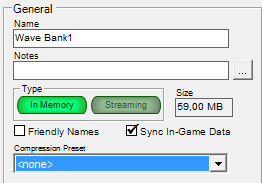
\includegraphics[scale=1]{images/compress-avant.png}
		\caption{Avant}
		\label{fig:image1}
		\end{center}
		\end{minipage}
		\hfill
		\begin{minipage}[c]{.45\linewidth}
		\begin{center}
		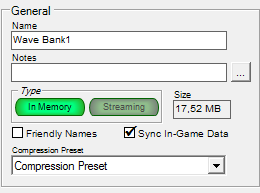
\includegraphics[scale=1]{images/compress-apres.png}
		\caption{Apres}
		\label{fig:image2}
		\end{center}
		\end{minipage}
	

		\vspace{4mm}
		
		
		
		\newpage
		
		
		\section{\'Etat de jeux}
		
		\vspace{5mm}
		
		Pour naviguer dans le jeu nous avons mis différents "États". Ces "États" sont les pages de menus, de selection du mode, les pages de jeux, etc.. 
		
		\vspace{8mm}
		
		\begin{center}
			\includegraphics[scale = 0.1]{images/Menus.png}
		\end{center}
		
		
		\vspace{10mm}
			 
			 
		
		Mais bien évidemment il faut des liens entre ces pages pour passer de l'une à l'autre. Dans les premiers jours de code, nous avons rencontré quelques difficultés dans l'agencement de ces états puisque tout était placé dans le Game1 et ce n'était donc vraiment pas simple de s'y retrouver et de modifier correctement les updates nécessaires et les bons affichages. En écoutant des étudiants de niveau supérieur, la solution la plus claire était de faire une pile d'état qui n'afficherait et ne mettrait à jour que le haut de la pile.\\
		
		Après des recherches, quelques tests et des ratés face à cette utilisation de pile, la combinaison d'une énumération d'états et d'un switch s'est avérée correspondre aussi bien à nos attentes. Cela nous a permis de simplifier au maximum le code dans le Game1 et de créer des Classes pour chaque état.\\
				
		\newpage	
			\begin{center}
						
\includegraphics[scale = 0.3]{images/blanc.png}
					\end{center}
		\noindent Morceau de code extrait de l'update() actuel du Game1 :
		
		
		\begin{mylisting}
	switch (CurrentGameState)
	{
		case GameState.MainMenu:
			MenuMain.Update(gameTime);
			break;
			
			.
			.
			.
			
		case GameState.Win:
			MenuWin.Update(gameTime);
			break;
	}
				\end{mylisting}
		
		\vspace{10mm}
		
		Avec cette configuration, chaque état a sa propre Classe. Le Game1 se retrouve donc largement simplifié puisqu'avec le switch il sait quel État actualiser ou afficher.\\
		
			
		C'est, comme vous l'aurez sans doute compris, dans le "GameState.Playing" que le gros du jeux va se passer puisque c'est ce qui correspond à une partie (dans un des deux modes).
		
		
		\vspace{10mm}
		\newpage
		
		
		
	\section{\'Editeur de Map}
						
			Nos cartes sont représentées avec différents chiffres correspondant à des blocs. Par exemple, lorsqu'il y a un "0", cela signifie qu'il y a une case vide à cet emplacement. Le second bloc à retenir est le "1". C'est lui qui représente la ligne d'arrivée (qui une fois franchie nous fait gagner) dans le mode histoire. Le "2" quand à lui va représenter le fameux bonbon que notre oiseau recherche tant et qui lui permettra de gagner à nouveau de l'énergie. Les autres blocs sont les obstacles infranchissables, ils n'y a pour l'instant que deux types d'obstacles. Nous n'utilisons donc que le "3" et le "4".\\
			
			\indent Maintenant que vous avez compris de quoi se compose une map, vous serez d'accord avec nous pour dire que les écrire à la main peut devenir terriblement long et très vite lassant. C'est pour cela que nous avons créé un éditeur de maps qui écrira lui même dans le fichier .lvl de façon à ce que nous ayons juste à cliquer un peu partout pour avoir une jolie map.
			
			\vspace{10mm}
			
	\noindent Screen de la bête : 
						
		\vspace{4mm}
		
			\begin{center}
			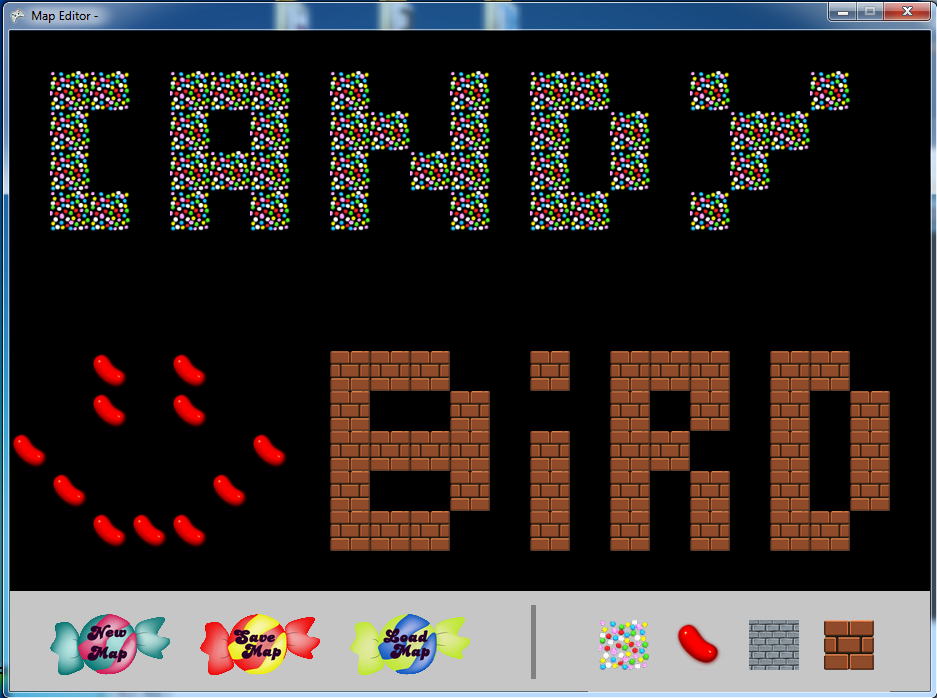
\includegraphics[scale = 0.4]{images/EditeurMap.png}
			\end{center}
			
			
			
		\newpage
			
			
			
			Nos Maps sont basées sur des fichiers textes (en .txt) que nous renommons en .lvl pour level (sans blagues). Le fichier est composé de:\\
						
						\indent- une première ligne indiquant le nombre de lignes de blocs où seront placés des \\\indent obstacles ou des bonbons.\\
						
						\indent- une deuxième ligne indiquant cette fois le nombre d'éléments à afficher sur chaque\\\indent ligne. C'est donc l'affichage horizontal du jeu.\\
						
						\indent- un ensemble de lignes de même longueur (que nous mesurerons pour la création de \\\indent la carte)et permettent de placer tous les éléments à différents emplacements sur la carte\\\indent selon la ligne ainsi que la colonne sur laquelle ils se positionnent.
						
						
						\vspace{10mm}
						
						\begin{center}
							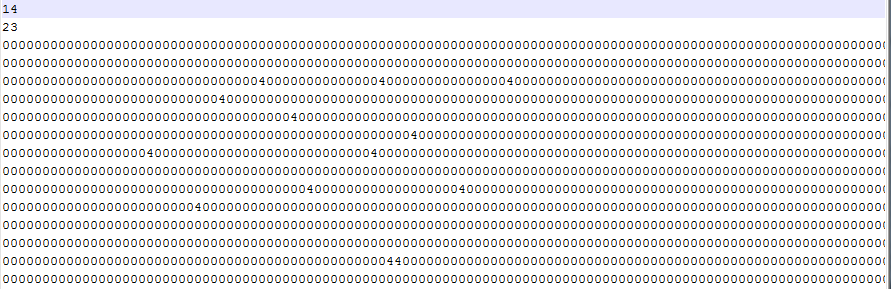
\includegraphics[scale = 0.6]{images/lvl.png}
						\end{center}
						
						\vspace{10mm}
			
			
		
			 	
			 \indent Lors de la création de l'éditeur de map nous avons eu différents problèmes. Tout d'abord lors de la création des éléments visuels tels que les boutons, n'ayant pas de graphiste dans le groupe, cette tache nous a pris plus de temps que prévu. Au niveau de la création de la partie fonctionnelle de l'éditeur de map, nous ne savions pas du tout comment nous y prendre. Puis, après avoir étudié nos besoins et ceux des utilisateurs, nous avons pu mettre en place les différentes parties de notre éditeur. Skeat et Vincae se sont partagé le travail.
			 
			 Vincae s'est occupé de toute la partie affichage des différents obstacles et bonbons afin de faciliter la vision d'ensemble d'un niveau ainsi que du chargement de maps existantes et de la sauvegarde des maps.\\
			 
			 
			 
	\newpage
		
	\noindent La fonction SaveMap : 
			 
	 \begin{mylisting}
	
      for (int j = 0; j < mapHeight; ++j)
      {
        if(j > 0)
           objWriter.WriteLine("");
        for (int i = 0; i < mapWidth; ++i)
        {
           objWriter.Write(layer[i, j]);
        }
      }
      
	\end{mylisting}
		
		
		\vspace{10mm}
		
		
		
		Dans cette partie du programme qui permet la sauvegarde d'une carte à partir de  notre éditeur, nous utilisons deux boucles imbriquées. La première gère les lignes tandis que la deuxième correspond à une place dans cette ligne (ce qui correspond donc aux colonnes).
		
		De cette manière, on parcourt la map dans sa totalité et pour chaque élément on va écrire dans le fichier .lvl la valeur du bloc lui correspondant contenu dans le tableau layer. 
		
		De plus, à chaque début de ligne, exceptée la première, on retourne à la ligne dans notre fichier pour que ce soit bien un bloc uniforme de ligne et non une grande ligne unique.\\
		
		\vspace{10mm}
		
		
		 Skeat s'est occupé de la modification en temps réel de la map. Cette partie consiste à récupérer le bloc que l'utilisateur sélectionne, et \`a placer à l'endroit souhaité sur la map. Une petite difficultée s'est posée sur cette partie puisqu'il est question de savoir où le clic a été effectué pour placer le bloc au bon endroit dans la matrice de la map puis l'afficher sous la souris, tous ca dans le but d'optimiser, et d'/'eviter que l'éditeur rame.\\
			 
			
	
	
	\newpage
	
	\section{Réseau}
	Comme expliqué dans l'introduction, notre jeu permet, si l'on se connecte au démarrage du jeux, d'envoyer le score à la base de données de notre site web.\\
	
	Avec quelques tutos en ligne et les connaissances de T4ze dans le domaine du Web, la compréhension des fonctions nécessaires fut assez simple et l'implémentation rapidement fonctionnelle.
	
	La gestion qui concerne la base de données (lecture, écriture, test) utilise une Dll nommée "Mysql.Data" car il n'est, par défaut, pas possible de faire communiquer un environnement de jeux en C\# avec une base de données en MySql. Cette Dll est disponible en téléchargement libre sur internet et se trouve très simplement; parfois même avec des exemples de fonctions. Mais nous avons préféré tout reprendre nous même pour avoir un code propre, optimisé et surtout que nous contrôlons entièrement.
	
	Pour la comprendre et pouvoir la contrôler sans faire planter notre jeux, nous avions préalablement implémenté la classe DBConnect.cs dans un projet annexe. Nous avons ainsi pu tester les fonctions d'ajout de données, de suppressions, de mises à jour, de tests d'existence de valeur et de listages au fur et à mesure qu'elles étaient écrites. Certaines fonctions créées ne nous sont pas utiles dans l'état actuel du jeu. Mais puisque nous étions sur notre lancée et dans une pensée d'améliorations possibles du jeux si nous voulons par la suite, par exemple, rajouter des options telles que s'inscrire depuis le jeux, afficher le classement ou encore changer de pseudo, elles seront déjà prête.\\
	
	\vspace{4mm}
	
	\noindent Forme de la base de données avec laquelle le jeux communique :
	\begin{center}
		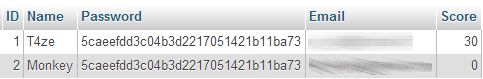
\includegraphics[scale = 0.8]{images/Bdd.png}
	\end{center}
		
		
	\vspace{10mm}
	
	Comme vous pouvez le voir sur le screen de la base de données, pour plus de sécurité nous chiffrons votre mot de pass en md5. De cette façon, même si un individu parvenait à s'infiltrer dans notre site (quasiment impossible vu notre sécurité), il ne pourrait pas modifier votre score, vous êtes donc bien protégé chez nous. C\# contient une méthode de chiffrement md5 qui nous facilite grandement le test de correspondance de mot de passe puisqu'à notre niveau, implémenter ce chiffrement aurait été vraiment compliqué.
	
		
	\newpage
	
	\begin{center}
			
\includegraphics[scale = 0.3]{images/blanc.png}
		\end{center}
	
	\noindent Toute cette partie nous sert à ceci : Le classement inter-joueur
	
	\begin{center}
		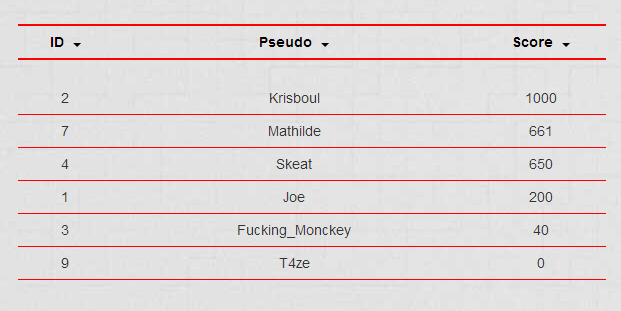
\includegraphics[scale = 0.6]{images/classement.png}
	\end{center}
			
	
	
	\vspace{10mm}

	L'envoi du score se fait uniquement en mode Map Infinie (le score ne se base que sur le nombre de mètres parcourus, il n'y a pas donc pas de score comptabilisé sur les maps prédéfinies). Cet envoi est réalisé en fin de partie, lorsque vous avez perdu et uniquement si vous vous étiez au préalable connecté à votre compte CandyBird. Cet enregistrement est obligatoire car sans lui vous n'existez pas dans la base de donnée et donc votre score n'est pas comptabilisé dans le classement.
	 
	 \newpage
	 
	\section{Site Web}
	
	\begin{center}
				
\includegraphics[scale = 0.3]{images/blanc.png}
			\end{center}
	
	\noindent URL du site web : 
	\begin{Verbatim}
	http://www.CandyBird.eu/
	\end{Verbatim}
	
	\vspace{6mm}
	
	Dans un esprit pédagogue, nous avons choisi de réaliser notre site à la main plutôt que d'utiliser un CMS (Wordpress ou autre). T4ze avait déjà, auparavant, monté différents site web et il a ainsi pu s'occuper de cette partie sans trop de problèmes.
	
	Le site regroupe actuellement une présentation rapide de notre projet accompagnée d'images qui illustrent les différentes parties de notre jeu. Chaque membre du groupe a sa page personnelle, avec une petite présentation ainsi qu'une photo (la classe). Pour la partie pratique, vous pouvez télécharger nos différents rapports, en LaTeX ou en PDF, ainsi que la version du code source présenté lors des différentes soutenances directement depuis le site. De plus, une page est réservée à l'inscription (avec enregistrement de carte bleu tout ça tout ça... histoire de rembourser tous nos frais de l'année). Cette partie n'est pas obligatoire mais recommandée puisque qu'il faut se connecter au jeux pour accéder au mode multijoueur et avoir l'envoi de score en ligne en fin de partie.\\
	\vspace{4mm}
	
	\begin{center}
	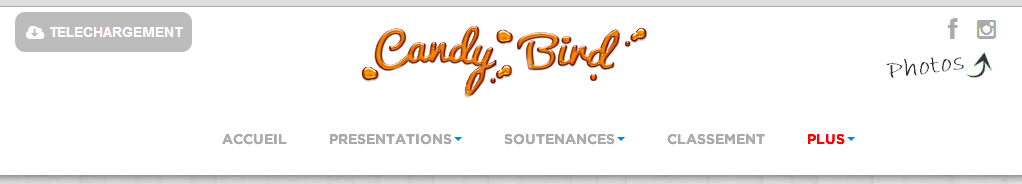
\includegraphics[scale=0.5]{images/site.png}
	\end{center}
	
	\vspace{10mm}
	
	Pour rester à l'écoute de nos admirateurs, une page de contact est disponible. Vous avez donc la possibilité de nous laisser des commentaires ou de nous suggérer des améliorations (pas de signalement de bugs puisque nous codons assez bien pour qu'il n'y en ai pas). Et pour ceux qui aiment être toujours informés, nous tenons une page facebook dont un raccourci est visible sur le site (à gauche dans le pied de page).
	
	\vspace{10mm}
	
	\newpage
	
	\section{Graphique}
	La partie graphique du projet a été compliquée suite au départ imprévu d'Adrien. C'était lui qui était le plus expérimenté face aux logiciels d'édition d'images (Photoshop en l'occurrence). Il a donc fallu  très vite apprendre les bases de ce logiciel afin de pouvoir réutiliser et modifier les travaux qu'avait déjà produit par Adrien. Ce petit problème n'était pas des moindres puisqu'un jeu avec des graphismes mal finis n'est pas très agréable à jouer et nous le savons bien.
	
	\indent Nous n'avons pas de personne directement assignée au graphisme, chacun crée les graphismes dont il a besoin au fur et à mesure que nous avançons dans nos parties. Ce n'est pas forcément très efficace mais cela évite qu'un des membres se consacre entièrement au graphisme au détriment du code car ce n'est pas un projet de graphisme. Nous souhaitons que chaque membre puisse apprendre ce qu'il souhaite, c'est pour cela que nous sommes parfois peut-être trop nombreux sur une même tâche, mais cette méthode a l'avantage d'impliquer l'ensemble de l'équipe \`a 100\% dans le projet.\\*
	\indent Nous avons tout de même défini et suivi un modèle de départ pour partir sur les mêmes bases afin de ne pas se retrouver avec des thèmes décalés d'une partie à l'autre. Chaque modification est montrée à tout les membres de l'équipe pour qu'ils puissent donner leur avis et valider ou non.
	
	\vspace{15mm}
	
	\subsection {Sprite}
	Le personnage principal n'étant pas tellement d'accord avec la façon dont on se sert de lui dans le jeux, bien qu'il ait fermé les yeux sur cette utilisation, il a préféré rester quelque peu dans l'ombre (ce qui explique son allure étonnement sombre et ses yeux fermés).
	La planche de sprites que nous utilisons provient de la source d'un projet qui a été annulé et rendu open source. Nous nous sommes permis de la récupérer et de la modifier à notre convenance.
	
	\vspace{4mm}
		
		\begin{center}
		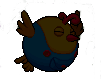
\includegraphics[scale=0.5]{images/bird.png}
		\end{center}
		
	\vspace{10mm}
		
	Le jeux étant en 2D, seul le profil de l'oiseau nous intéresse. Le personnage est donc géré via un spritesheet, une image qui comporte les détails des mouvements du personnage. Six animations s'enchainent en boucle pour faire bouger ses ailes et ses pattes rendant ainsi son vole plus réaliste.
	
	
\newpage
	\section{Répartitions des Tâches}
	\vspace{8mm}
	\begin{center}
			\begin{tabular}{| l |*{4} {c|}}
				\hline
				Themes  & Mathilde & Florent & Thibault & Vincent \\
				\hline
				Son     & X &         & X    &        \\
				\hline
				Réseaux       &     & X       &       & X     \\
				\hline
				Mode Histoire     & X &     & X      &       \\
				\hline
				Mode Infini         & X &      &     &          \\
				\hline
				Menu et \'Etats        &  & X    &  &          \\
								\hline
				Moteur Physique & X      & X        & X &           \\
				\hline
				Editeur de Map &     &       & X     &  X\\
				\hline
				Site Internet  &    & X &     &  X       \\
				\hline
				Graphisme      & X  &  X  &         &\\
				\hline
				Courses/Repas      & X  &  X  &  X  & X\\
				\hline
				Vaisselle      & X  &     &         &\\
				\hline
				
			\end{tabular}\\\vspace{3mm}
	\end{center}
	
	\vspace{10mm}
	
	\section{Les chiffres}
	\vspace{8mm}
		\begin{center}
				\begin{tabular}{| l |*{4} {c|}}
				\hline
				Bières & 50€ \\
				\hline
				Consommation électricité & 400 MW  \\
				\hline
				Consommation d'eau & 1 douche par jour (x4)  \\
				\hline
				Nourriture & 250€ \\
				\hline
				Code & 27 429 lignes  \\
				\hline
				Erreurs stupides & un gros paquet  \\
				\hline
					
				\end{tabular}\\\vspace{3mm}
		\end{center}
	
	
\chapter{Et Après?}
	\section{Map Editor 2.0}
	L'éditeur de map sera intégré au jeu afin que vous puissiez créer vos propres maps et ainsi étendre la durée de vie de notre jeu (qui est déjà infinie), vous aurez aussi la possibilité de mettre au défi vos amis en partageant vos créations, ce qui rendra le jeu quelque peu plus addictif.
	
	
		
		\vspace{10mm}
	
	
	
	\section{Réseaux Multijoueurs}
	Nous allons encore ajouter un mode de jeu qui sera un vrai mode multijoueurs, o\'u vous pourrez jouer directement contre un de vos amis, en \'etant sur la m\^eme map. Sur ce mode de jeu vous ne pourrez pas mourrir, pour gagner la partie il faudra passer la ligne d'arriv\'ee en premier. Pour vous aider aller plus vite des bonbons magiques se trouveront sur la map, qui pourront vous faire traverser les blocs, aller plus vite, mais attention au pi\`eges certains bonbons pourront \^etre empoisone est donc vous ralentir.

	
	\vspace{10mm}



	\section{Nouveaux Personnages}
	Nous savons que notre bel oiseau est très attachant, mais nous avons décidé de rajouter de nouveaux personnages, qui auront des caractéristiques physiques différentes, pour que vous puissiez choisir un personnage qui vous corresponde le mieux possible.
	
	
		
		\vspace{10mm}
	
	
	
	\section{Graphismes}
	Au niveau graphismes pour la suite nous comptons cr\'eer de nouveaux sprites de personnages, nous allons aussi refaire des fonds de maps afin de rendre le jeu encore plus divertissant. Nous allons aussi rajouter des blocs de différents styles pour que les décors et les blocs se trouvant sur la même map soit sur le même style, et garder ainsi une certaine homogénéité dans les décors
\newpage

\chapter*{Conclusion}
\addcontentsline{toc}{chapter}{Conclusion}

Après un premier semestre de travail intense, nous pouvons ainsi dire que nous suivons la progression prévue. Nous approchons de plus en plus d'un rendu jouable. Notre ambition a été mise à l'épreuve mais notre motivation nous a permis de garder le moral et d'arriver à nos fins. Nous conservons tout de même notre idée de départ qui est de présenter à la fin de la soutenance finale un jeu complet, totalement fonctionnel et, pourquoi pas, le distribuer à un maximum de joueurs.\\

Cette première partie nous a permis d'évaluer la quantité de travail à fournir pour les prévisions que l'on fait pour la suite, mais cette quantité de travail ne nous effraie plus. Nous somme très fiers des réalisations de notre groupe ainsi que de l'ambiance qui y règne.\\

Nous espérons que notre jeu vous plaira et que nous serons capable de vous épater par ses améliorations.\\


\vspace{10mm}
		
		\begin{center}
		
\includegraphics[scale=1.3]{images/birdfin.png}
		\end{center}




\end {document}